\subsection{MARCO TEÓRICO}

Esta parte del capítulo expone el contenido teórico necesario para la
realización de este proyecto. Esto incluye información sobre los motores
eléctricos,  análisis de la vibración, las herramientas computacionales, los
sistemas y el modelado estadístico.

%https://es.wikipedia.org/wiki/Motor_el%C3%A9ctrico


\subsubsection{ Motores eléctricos}

De acuerdo a \textcite{Fraile}, un motor eléctrico es un dispositivo que
transforma energía eléctrica en
energía mecánica mediante la acción de campos magnéticos y están compuestos,
principalmente, por un estator (parte fija) y un rotor (parte móvil).
Existen dos familias principales de motores eléctricos las cuales, a su vez,
se subdividen en \textbf{motores de corriente alterna} como lo son los  motores
de inducción, síncronas, entre otros y los \textbf{motores de corriente continua}
como lo son los motores de escobillas,  sin escobillas, de imán permanente,
entre otros.

El motor más usado, en el sector industrial, es el motor de inducción debido
principalmente a su bajo costo y al poco mantenimiento que requiere para estar
completamente operativo, esto en particular es debido a su sencillo diseño
en comparación al de otros motores de igual potencia, ya que requiere  menor
número de componentes. Cabe resaltar que el segundo tipo de motor más usado es
el motor de corriente
continua, debido a que su control, en términos de torque y potencia, es mucho
mas sencillo para ciertos niveles de potencia.

También existen los motores síncronos, cuya construcción es similar a la de un
motor de inducción pero a su vez requiere de una fuente de alimentación externa
para el rotor, lo cual aumenta su costo, además de esto su velocidad es
constante, por lo tanto este tipo de motor es utilizado en aplicaciones
específicas. Como se mencionó anteriormente, existen otros tipos de motores,
pero son usualmente de menor potencia por
lo tanto su utilidad industrial es mucho más limitada.


\subsubsection*{Rodamientos}

Para que un motor pueda llevar a cabo la transformación de potencia debe rotar.
Esta acción es llevada a cabo por el \textbf{rotor}, el cual esta formado por un
eje que soporta un juego de bobinas envueltas sobre un núcleo magnético. Este
se encuentra suspendido por \textbf{rodamientos}, de forma que el movimiento y
las fuerzas producidas en la interacción entre las bobinas y el núcleo con los
campos magnéticos, producidos por el estator, puedan ser utilizados. Además,
los rodamientos, cuando se encuentran en buenas condiciones, permiten minimizar
el roce entre el eje y soporte, maximizando la transferencia de potencia.

Estos también son conocidos como \textbf{rolineras}, las cuales según
\textcite{rodamiento},  son un tipo de cojinete,
un elemento mecánico diseñado para reducir la fricción entre un eje y los
elementos conectados al mismo. Existen muchos tipos de rolineras, sin embargo
su estructura se fundamenta en dos anillos concéntricos, algún elemento rotativo
como pueden ser bolas o rodillos, una jaula que se encarga de mantener los
elementos de rodadura separados además de guiados y un lubricante o un sistema
de lubricación.

Dado que son un elemento mecánico, el cual es continuamente usado, sufre mucho
desgaste y es el elemento más propenso a dañarse; según los estudios realizados
por ~\textcite{Kammermann} el 59\% de las fallas son causadas por los rodamientos
y asimismo su principal falla es el desgaste, de igual forma se presentan
otras fallas estructurales. Por estas razones es fundamental tener bajo continuo
monitoreo este elemento, esto se suele hacer a través de un análisis de vibración.


\subsubsection{Análisis de Vibración}

Como se explica en \textcite{wiki:Vibration}, la vibración es el  movimiento
periódico de un cuerpo o medio
elástico, alrededor de un punto de equilibrio. En general podemos decir que una
vibración es un caso específico de una oscilación, cuando esta es de origen
mecánico.

Asimismo, se conoce como análisis de vibración, al conjunto de técnicas que permite
obtener información de un equipo, a partir de sus vibraciones. Es una de las
técnicas más usadas en el mantenimiento predictivo de equipos mecánicos, debido
a que es un proceso poco invasivo y de bajo costo. El análisis de vibración
permite diagnosticar fallas de forma temprana, así como detectar señales
prematuras de desgaste.

Según Girdhar \textcite{Girdhar},  el análisis de vibración nos permite detectar las
siguientes fallas:

\begin{itemize}[noitemsep]

\item Defectos en los engranajes
\item Defectos en los rodamientos
\item Desalineamientos
\item Desbalances
\item Ejes torcidos
\item Excentricidad
\item Fallas eléctricas
\item Fuerzas hidráulicas o aerodinámicas
\item Mala sujeción en las piezas
\item Problemas en las correas de transmisión
\item Problemas de lubricación
\item Resonancia
\item Rozamientos en el rotor
\end{itemize}


\subsubsection*{Adquisición de datos}

Para realizar cualquier tipo de análisis, primero se deben adquirir datos y,
por regla general, mientras más datos se tengan y más precisas sean las
mediciones, mejores serán los estudios que se pueden realizar.


La adquisición de datos, según \textcite{adquisiciondatos}, es el proceso de
realizar mediciones de fenómenos físicos
y registrarlos, en algún formato específico, para analizarlos posteriormente.
Cabe resaltar que en algunos casos es necesario hacer un acondicionamiento de
la señal, esto
implica modificarla controladamente al reducir o aumentar su amplitud además de
sumarle un nivel offset, voltaje continuo, para que cumpla requisitos mínimos
y pueda ser procesada por los siguientes circuitos.

Al momento de la adquisición de datos, se toman medidas de una señal analógica
la cual se convertirá al pasar por una serie de etapas y dispositivos en una
señal digital y se guardará en un formato deseado y en una unidad de
almacenamiento masivo (ROM, flash, etc.).
El primer paso en la toma de  datos comienza con el sensor, que es un
dispositivo el cual transforma la unidad física de interés, en una señal que
pueda ser procesada con mayor facilidad, luego se adecuará mediante un
circuito especializado a las características y requerimientos del sistema,
posteriormente será procesada por un convertidor Analógico-Digital, el cual se encarga de
muestrear, retener y procesarla  y, de esta forma, obtener una versión
digital de la misma, la cual se  guardará mediante un software desde
una computadora.

En el caso de las vibraciones, los sensores más usados son los
acelerómetros.  Esto se debe principalmente a que tienen mayor ancho de banda
que los sensores de posición y los de velocidad, lo que les permite detectar
vibraciones de mayor frecuencia. Adicionalmente, dado que las vibraciones en los
rodamientos, por naturaleza, son de alta frecuencia y, como se mencionó anteriormente,
son componentes críticos en los motores eléctricos.
Estas características hacen al acelerómetro el sensor más utilizado para las
mediciones de vibración en motores eléctricos. Sin embargo,
en casos más especializados, como podría ser el análisis de vibración
de maquinaria de larga envergadura, son también usados los otros tipos de
sensores ya que sus características pueden facilitar el estudio.


\subsubsection{Acelerómetros}

Como se expone en \textcite{Fraden}, un acelerómetro es un dispositivo capaz de
medir aceleración, no es
necesariamente la misma que la aceleración de coordenadas (cambio de la velocidad de
un elemento en el espacio), sino que es la correlación asociada con el fenómeno
de peso experimentado por una masa de prueba que se
encuentra en el marco de referencia del dispositivo.  Funciona mediante
la utilización de la segunda ley de Newton, \textbf{la fuerza resultante
ejercida sobre un cuerpo es proporcional a su masa por su aceleración}. Los
acelerómetros por lo general cuentan con una masa de prueba (también conocida
como masa sísmica), alguna especie de resorte y un marco de soporte que, a su
vez, puede funcionar como amortiguador. Debido a esto, los acelerómetros se
pueden modelar matemáticamente como un sistema lineal de segundo orden,
por lo que su respuesta en frecuencia posee un pico de resonancia.


\subsubsection*{Tipos de acelerómetros}

\begin{itemize}
    \item  Acelerómetros Capacitivos:

        Los acelerómetros capacitivos son uno de los modelos más sencillos
        capaces de medir
        aceleración, además de ser fácilmente utilizables y reproducibles en masa.
        Funcionan mediante una masa sísmica dado que al  experimentar una fuerza
        se desplaza con una aceleración proporcional a la fuerza aplicada.
        Si a la masa se le agregan unos resortes unidos a una carcasa, los resortes
        ejercerán una fuerza proporcional al desplazamiento de la masa generando un
        desplazamiento fácilmente medible.

        Este fenómeno se produce ya que estos efectos en conjunto al
        amortiguamiento producen un sistema lineal de
        segundo orden, este sistema matemático genera una salida en desplazamiento
        al aplicarse como entrada una fuerza
         Finalmente, al conectarse un sensor de desplazamiento, se observa
        la aceleración a la que esta sometido el instrumento.
        El sensor de desplazamiento más
        popular para este tipo de medidores es el capacitivo.

        En su mayoría, los acelerómetros capacitivos vienen como dispositivos
        microelectromecánicos (\textbf{mems} por sus siglas en inglés) que son
        dispositivos
        fabricados con técnicas similares a las de fabricación de circuitos
        integrados; a su vez, poseen componentes mecánicos microscópicos. Son los
        acelerómetros más populares en aplicaciones no industriales, sin embargo,
        en aplicaciones de bajo consumo, bajo coste o cuando las frecuencias con
        las que se trabajan no son tan altas, pueden ser usados a niveles
        industriales, ya que poseen múltiples ventajas como:

        \begin{itemize}[noitemsep]
            \item No requieren adecuación de la señal.
            \item Pueden comunicarse directamente con un microcontrolador.
            \item Su precio es económico.
            \item Son compactos.
        \end{itemize}


    \item  Acelerómetros piezoresistivos:

        Son, después de los acelerómetros piezoeléctricos, los más usados a nivel
        industrial. Su funcionamiento es similar al de los acelerómetros
        capacitivos; ante una aceleración de entrada se produce un desplazamiento
        de salida más, en este caso, están constituidos por una o varias
        galgas extensiométricas, una masa de prueba y unos resortes de soporte.
        La galga sujeta a la masa sísmica y, al esta recibir una fuerza, produce
        un desplazamiento proporcional a la fuerza aplicada, lo que deforma a
        su vez la galga extensiométrica lo cual se traduce como un
        cambio de resistencia en el sensor. La ventaja de los acelerómetros
        piezoresistivos es que pueden medir valores de voltaje DC lo que los
        hace útil en el estudio de impactos, son también usados en el
        análisis de vibración en el rango de mediana frecuencia.

\newpage
    \item Acelerómetros piezoeléctricos:

        Según \textcite{WeberPiezoelectricAT}, es el acelerómetro más usado en
        aplicaciones industriales ya que
        poseen características como:

        \begin{itemize}[noitemsep]
            \item Alto rango dinámico.
            \item Bajos niveles de ruido.
            \item Alta linealidad.
            \item Alto ancho de banda.
            \item Poco desgaste, ya que no poseen partes móviles.
        \end{itemize}


        Su construcción es bastante sencilla, se tiene disco de un cristal
        piezoeléctrico unido por dos terminales circulares, de forma similar a
        la de un condensador, y justo encima, tienen una masa de prueba.
        Al experimentar una fuerza el cristal se deforma lo que produce una
        diferencia de carga y un voltaje proporcional a la fuerza aplicada.
        Como la aceleración de la masa de prueba es también proporcional a la
        fuerza aplicada, la aceleración del acelerómetro será entonces
        directamente proporcional al voltaje y la carga producida en el cristal.

\end{itemize}


\subsubsection{Procesamiento de señales}

Después de ser almacenada la información, debe ser estudiada, procesada, para lo
cual se utiliza una serie de herramientas, técnicas o software especializados
a cada necesidad. Este estudio se puede categorizar en dos ramas principales:

\begin{itemize}
    \item Dominio del tiempo, según \textcite{wiki:DominioTiempo}, es un término
        utilizado para describir el análisis
        de funciones matemáticas o señales con respecto al tiempo, la sucesión
        de estados que atraviesa la señal de forma natural. Los estudios más
        comunes son en  \textbf{tiempo continuo} y en \textbf{tiempo discreto}.

    \item Dominio de la frecuencia, según \textcite{wiki:DominioFrecuencia}, es un
        término utilizado para describir el análisis
        de funciones matemáticas, señales o movimientos periódicos respecto a
        su frecuencia, número de veces que sucede un evento en un periodo.
        Utilizan transformadas para llevar las funciones o señales del dominio
        del tiempo, base, al dominio de la frecuencia, deseado, la más famosa es
        la \textbf{transformada de Fourier}.
\end{itemize}


Gráficamente se suele entender el \textbf{dominio temporal} como la evolución
de una señal con respecto al tiempo, es decir su evolución natural, por otro
lado, el \textbf{dominio frecuencial} muestra los componentes de la señal según
la frecuencia en la que oscilan dentro de un rango determinado.
En la figura \ref{Dominios} se observan ejemplos gráficos de señales en ambos
dominios.

	\begin{figure}[htb]
		\centering
        \caption{ Diagrama de los dominios temporal y frecuencial}
        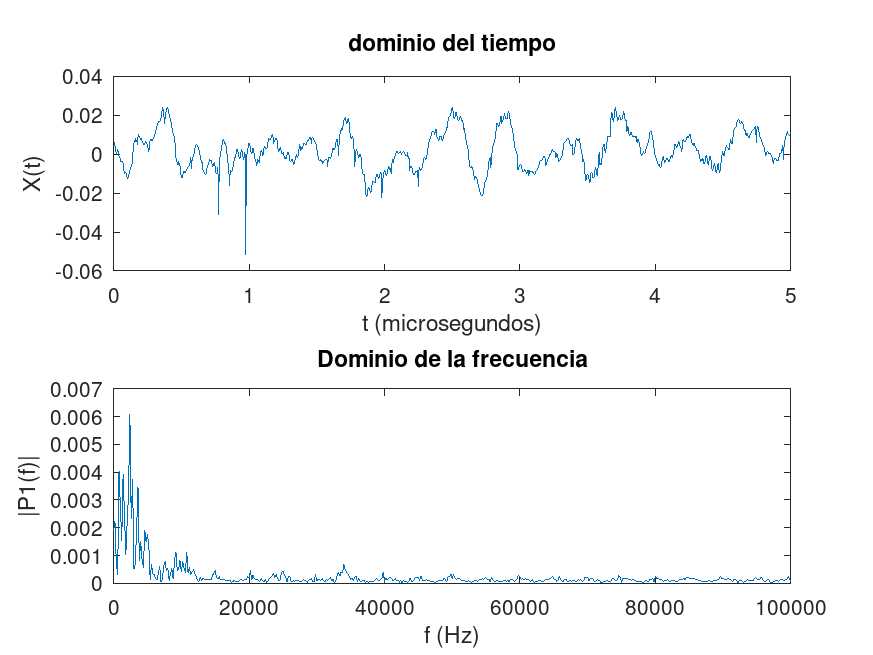
\includegraphics[width=\linewidth]{Dominios.png}
        Realizada con el Software Octave a partir de los datos de
                \textcite{HUANG20181745}
        \label{Dominios}

	\end{figure}


El análisis en frecuencia suele ser más utilizado debido a que
la mayoría de las fallas poseen frecuencias características y, dado que en  el
análisis de frecuencia se descompone en frecuencias la señal, se facilita la
detección de fallas características, así mismo, la amplitud de la frecuencia es
directamente proporcional al nivel de la falla. Por lo tanto, se obtiene un
espectro amplio del estado de la pieza.
Cabe resaltar que cuando las frecuencias son bajas o muy cercanas entre si,
se dificulta determinar e identificar alguna falla, suele suceder cuando se
estudia una falla o evento con frecuencia muy baja o muy cercana a la frecuencia
natural de la señal o elemento medido. En estos casos es mejor
usar un análisis en el dominio del tiempo que  facilita la
detección de las fallas.



\subsubsection{Herramienta Computacional}


Según \textcite{Herramienta}, una herramienta computacional puede ser definida  como
cualquier software,
sistema de integración, análisis o almacenamiento que  ayuda a los científicos
o usuarios a solucionar un problema específico en una determinada rama. Pueden
variar desde sistemas complejos como compiladores, algoritmos
e incluso sistemas operativos hasta herramientas como hojas de cálculos, sistemas
de oficina o medios de comunicación. Funcionan mediante la implementación de
técnicas y protocolos para solucionar problemas de forma iterativa o con una
secuencia de pasos concreta.

Siguiendo este orden de ideas, una gran cantidad de estas herramientas son
encontradas en la librería de información más grande del mundo, el Internet.
Todas comparten la peculiaridad de que son un \textbf{sistema} y,  por ende, pueden
ser accedidas con facilidad desde cualquier punto con un dispositivo capaz de
tener conexión a Internet y un navegador. Esta facilidad se debe a que un
\textbf{servidor} se encarga de hacer el procesamiento de la información y envía
el resultado con un formato específico, típicamente  JSON, por \comillas{notación de
objeto de JavaScript} el cual es un formato de texto sencillo para el intercambio de
datos, este se renderiza (proceso para generar una representación gráfica por
medio de programas informáticos) en una página Web.

\subsubsection{Sistema Web}

Los sistemas Web, de acuerdo a \textcite{SistWeb1} y \textcite{wiki:systemWeb}, o
también conocidos como aplicaciones Web son sistemas que
utilizan la tecnología Web y el Internet o Intranet para transmitir la
información y los
servicios a usuarios u otros sistemas/aplicaciones. Estos sistemas utilizan los
principios del hipertexto para renderizar la información en cualquier
navegador o \textbf{página Web} y el poder de los \textbf{servidores} para
almacenar y procesar la información. Por estas características son independientes
de cualquier plataforma o sistema operativo, además de  no requerir ningún
proceso de instalación, facilitando de esta forma el acceso, la gestión y la
rapidez de obtención de información.



\subsubsection*{Página Web}
Una página Web, como se explica en \textcite{WebpageMozila},  es un documento
accesible desde cualquier navegador con acceso
a Internet que puede incluir audio, vídeo, texto y sus diferentes
combinaciones.
Funciona al usar el protocolo HTTP, conocido usualmente como la Web, y una
estructura de hipertexto la cual permite redirigir, enlazar y estructurar el
contenido y lo hace fácilmente accesible desde un navegador Web.

Funciona gracias al protocolo HTTP, \comillas{Hypertext Transfer Protocol},
el cual es la base de cualquier intercambio de datos en la Web y un protocolo
de estructura cliente-servidor, esto implica que una petición de datos es
iniciada por el elemento que recibirá los datos (el cliente), normalmente un
navegador Web, y es cubierta por el elemento que envía los datos (el servidor).
Este protocolo comenzó siendo estático y dirigido usualmente a la transmisión de
texto pero se fue convirtiendo en más que eso y, en la actualidad, permite la
transferencia de documentos de todo tipo, Scripts, vídeos, entre otros; a tal
punto que es fácilmente categorizado como el protocolo más usado en todo el
mundo, siendo incluso utilizado como sinónimo de Internet cuando es solo una
parte de él.

Debido a la invención de tecnologías, como JavaScript y AJAX, hoy en día es
posible tener aplicaciones Web que son programas, junto a una interfaz gráfica,
que permiten comunicarse con servidores que realizan la mayor parte del trabajo
del desarrollo de aplicaciones complejas que funcionen desde la
comodidad de dispositivos móviles. La Web permite, por tanto, facilidad al
transmitir información así como el acceso a cualquier contenido desde
cualquier dispositivo, en cualquier momento.

La Web suele ser el método de acceso de muchas tecnologías y, si bien en la actualidad
el desarrollo Web usa el mismo estándar de tecnologías, el lado del servidor
contempla una variedad mucho más amplia, dado que cualquier aplicación que
pueda correr en un ordenador puede ser conectada a una interfaz Web. Teniendo
como limitante principal la latencia,  tiempo que tarda la información en viajar,
una interfaz Web es, para un usuario promedio, una solución cómoda y
accesible la cual  permite incluso  mayor comodidad y facilidad de acceso.


\subsubsection*{Servidor}

Un servidor Web, como lo define \textcite{servidor},  es un ordenador de propósito
específico que permite la
transición de datos a uno o múltiples clientes Web. Para esto, el dispositivo
debe estar configurado para escuchar las solicitudes de los clientes en un
entorno red. Esto se logra mediante una aplicación externa o el uso de un
sistema operativo dedicado; almacena los archivos
necesarios para el procesamiento de información y los datos necesarios para
mostrarla, además, se encarga de distribuirla al usuario final.

Los servidores se suelen clasificar según su función y es común que cumplan más
de una función, o se encuentren más de un tipo en una red. Algunos de estos son
servidores de archivos, impresión, aplicaciones, DNS, \textbf{Web}, entre otros.
Actualmente, los servidores Web son los más abundantes en el mercado
y se caracterizan por alojar la información y los datos de los usuarios a través
de Internet o Intranet. Estos responden a las solicitudes de páginas Web u otros
servidores basados en esta tecnología.

\subsubsection{Base de datos (BBDD)}
Una base de datos como dice \textcite{bbdd} es una herramienta para almacenar y
organizar información.
Las bases de datos pueden contener información de cualquier tipo
y se utiliza para evitar problemas como redundancia y para facilitar el manejo de
grandes cantidades de la misma, en fin,  una base de datos
computarizada es un contenedor de objetos la cual permite:

\begin{itemize}
    \item Agregar nuevos elementos.
    \item Editar y mover información en la base de datos.
    \item Eliminar información.
    \item Organizarla y visualizarla de diferentes formas.
    \item Compartirla con otros usuarios, programadores o interesados.
\end{itemize}

Las bases de datos, según \textcite{bbddTipos} se suelen dividir en dos tipos, de
acuerdo al tipo de lenguaje
utilizado para manipularlo, estas son SQL( ``Structured Query Languaje" utilizado
para bases de datos relacionales) y NoSQL (Sus tipos de datos no suelen ser
estructurados, aunque algunas bases de datos permiten su estructuración); su
utilización o selección depende mucho del tipo de procesamiento que se le
dará a la información contenida en ella, algunos otros factores importantes
a considerar son la velocidad de escritura-lectura y paralelismo.

\subsubsection{MongoDB}
MongoDB según \textcite{MongoDB} es un sistema de base de datos no relacional de código
abierto el cual utiliza documentos flexibles en lugar de tablas y columnas para
almacenar y procesar varios tipos de información. Al ser una solución NoSQL,
MongoDB no requiere un sistema de manejo relacional permitiendo esto un modelado
mas elástico al momento de guardar la información, además, permite mas libertad
en las consultas lo cual, además de simplificar el manejo para los desarrolladores,
permite desarrollar un ecosistema fácilmente escalable en aplicaciones y servicios
multi plataformas.

Cabe resaltar que el modelo de estructuración de datos que utiliza MongoDB es
BSON el cual es formato binario de JSON.

\subsubsection{MongoDB Atlas}
Como \textcite{MongoDBAtlas} especifica en su documentación oficial, MongoDB Atlas
es un servicio de base de datos (Database-as-a-Server, DBaaS) el cual permite
establecer, llevar a producción y escalar las bases de datos sin preocuparse por
el hardware físico, actualizaciones de software y los detalles de configuración.

Es decir, MongoDB Atlas es un sistema completamente manejado en la nube el cual
maneja toda la complejidad de llevar a producción el sistema, manejarlo y revisar
el estado de sus componentes, además, permite la utilización de cualquier proveedor
de servicios (AWS,Azure y GCP).

Cabe resaltar que MongoDB Atlas es un servicio pago, sin embargo, permite la
utilización de un ``cluster" gratuito, de almacenamiento limitado, para
prácticas y aprendizaje.

\subsubsection{Interfaz de programación de aplicaciones (API)}
Interfaz de programación de aplicaciones es una forma de simplificar el diseño
de software al permitir el intercambio de información y funcionalidades de forma
rápida y segura. Como explica \textcite{API} una API permite a las compañías y
desarrolladores abrir y expandir las informaciones y funcionalidades que poseen
con grupos externos de desarrolladores, compañeros de negocios e incluso departamentos
internos dentro de la misma compañía, esto permite separar los desarrollos y
trabajar de forma paralela ya que los desarrolladores no necesitan conocer la
implementación, simplemente la utilizan como interfaz para comunicarse con otros
productos y servicios.

Cabe resaltar que sin estas fuera imposible el desarrollo de muchas aplicaciones
populares. Una API funciona al ser un conjunto de normas que definen como se
comunicarán las computadoras o aplicaciones entre ellas, es decir, sirve como
una capa de abstracción entre el servidor y la aplicación.

\subsubsection{Modelo estadístico}

Un modelo estadístico, de acuerdo a \textcite{modeloIBM}, es una representación
matemática que permite, mediante
ecuaciones, codificar información extraída de los datos y, de esta forma,
predecir el comportamiento de un sistema ante situaciones dadas. Funcionan
mediante  variables aleatorias, una o más variables de las cuales no
se tiene completa certeza de su valor o provienen de algún evento aleatorio.

Un modelo estadístico permite inferir ciertas características de un evento,
como qué tan probable es tal evento y cómo se distribuyen los valores de la
variable. Además, se suele usar como primer paso en generar un modelo más
preciso o para la obtención de información cuando no se tiene suficiente,
es difícil su acceso o la naturaleza del
sistema es extremadamente compleja y dicha tarea es simplemente imposible.


\subsubsection{Lenguaje de programación}
Los lenguajes de programación pueden ser definidos, según \textcite{ETAC} como
sistemas estructurados
que permiten a las personas o programadores interactuar y dar instrucciones a un
programa o software con la finalidad de lograr objetivos.

En la actualidad existe una gran cantidad de lenguajes de programación, algunos
desarrollados en la antigüedad que todavía desarrollan un papel importante en
los sistemas, como lo son C, C++, Java y otros más modernos como lo pueden ser
Go, Rust y Python.

Como se explica en \textcite{javaTpoint}
Los lenguajes de programación suelen ser clasificados en bajo nivel y alto nivel,
haciendo referencia a la necesidad de un compilador o intérprete para poder ser
ejecutado por la computadora, siendo los de bajo nivel lenguaje de máquina o
ensamblador y los de alto nivel los lenguajes comúnmente conocidos, como
Python, Java, JavaScript, PHP, C++, Objective C, Cobol, Perl, Pascal, LISP,
FORTRAN, Go y Swift. Estos lenguajes de alto nivel se pueden subdividir
de acuerdo a la necesidad de un compilador (C,C++,Go, etc.) o de un intérprete
(Python, JavaScript, Ruby, etc.) en \textcite{LenguajesCompiladosEInterpretados}, se
puede leer más de esto. Asimismo, existe otra pequeña subdivisión en el ``tipado"
del lenguaje, que es la necesidad de especificar el tipo de valor que una
variable o constante puede tomar, siendo estas posibilidades un tipado fuerte,
medio o débil, también llamados dinámico (débil) o estático (fuerte).


\subsubsection{Go}
Go es un lenguaje de programación creado en 2007 en google, específicamente por
Robert Griesemer, Rob Pike y Ken Thompson, su sintaxis es similar a la del lenguaje
C y tiende a ser dinámico como Python pero con un rendimiento equiparable a los
de C o C++. Como se especifica en su página y documentación oficial
\textcite{GolangDocumentacion}: Go es un proyecto de código abierto (open source)
y gratuito
para hacer a los programadores más productivos, es un lenguaje expresivo, conciso,
limpio y eficiente con mecanismos de concurrencia (paralelismo) que permiten fácilmente
obtener el máximo rendimiento posible de las máquinas multinúcleo y redes de máquinas
actuales, mientras permite una programación flexible y modular, además de un compilado
rápido con un recolector de basura (el lenguaje se encarga de liberar memoria
no utilizada).
Es un lenguaje compilado rápido y con tipado estático (las variables y sus tipos tienen que
ser definidos con anterioridad) que se siente como un lenguaje interpretado y
con tipado dinámico (variables modificables sin tipo definido, más sencillo de
escribir el código pero menos estructurado).

Adicional a esto, este lenguaje tiene un ecosistema de comunidades, librerías y
herramientas en constante crecimiento que facilitan el aprendizaje y el desarrollo
de código.

\subsubsection{Fyne}

Fyne es una de las librerías (conjunto de herramientas o paquete) más utilizado
en Go para el desarrollo de interfaces graficas de usuario (GUI), como se
indica en su página oficial \textcite{fyne}
el conjunto de herramientas de Fyne es una herramienta fácil de aprender, gratuita
y de código abierto (open source) que permite la creación de aplicaciones gráficas
para escritorios, teléfonos y más. Combina el poder y la simplicidad del lenguaje
Go con una cuidadosamente creada librería de Widgets (miniaplicaciones o herramientas)
que hacen ahora más fácil que nunca la construcción de aplicaciones y su despliegue
a producción en todas las plataformas (sistemas operativos, ios, linux, windows, etc.)
y tiendas (windows store, google play, etc.).

\subsubsection{HTML}

HTML no es considerado un lenguaje de programación propiamente dicho por su
incapacidad de realizar acciones de lógica o aritmética, más específicamente y
de acuerdo a \textcite{HTML},
es un lenguaje de enmaquetado (una forma de escritura que utiliza elementos
sintácticos para dar forma y estructura a la información escrita posteriormente
a un proceso de  compilación o interpretación por la máquina, otros ejemplos son
Latex y Markdown), específicamente un lenguaje de enmaquetado de hipertexto y es
el bloque más básico para la Web ya que define y estructura el contenido de la
misma.

``Hipertexto"\  se refiere a los enlaces que se utilizan para conectar la página
Web con otras partes, ya sean de la misma página o paginas externas a la misma.
Estos enlaces son fundamentales en la Web ya que permiten la actualización y el
entrelazamiento de las páginas creadas por otras personas, esto permite
una participación activa el la\  ``World Wide Web".

HTML usa ``etiquetas"\  para dar información adicional  el texto, las imágenes,
el contenido y permitir
una correcta muestra del contenido, estos elementos sintaxicos son por ejemplo:
 <head>, <title>, <body>, <header>, <footer>, <article>, <section>, <p>, <div>,
 <span>, <img>, <aside>, <audio>, <canvas>, <datalist>, <details>, <embed>,
 <nav>, <output>, <progress>, <video>, <ul>, <ol>, <li>, entre otros.

 De esta forma, el mismo texto entre etiquetas distintas, va a tener características
 visuales distintas, por ejemplo, <h1>Algo<h1> es un título, negritas y tamaño de
 fuente muy superior a <p>Algo<p> que sería un párrafo.


\subsubsection{CSS}

CSS al igual que HTML no es considerado un lenguaje de programación, por las mismas
razones, en cambio, como se describe en \textcite{CSS} es una hoja de estilos en cascada,
un lenguaje utilizado para describir y dar estilo a documentos escritos en HTML o
XML, esto lo consigue al describir cómo los elementos deberían ser mostrados en la
pantalla, papel, habla u otra tipo de multimedia.

Dado estas características CSS es una parte fundamental en el desarrollo Web, ya
sea en su versión para o con la inclusión de Frameworks o librerías como lo son
Bootstrap o TailWind CSS.

Funciona mediante la especificación y modificación de las características en
entornos, etiquetas o elementos únicos, mediante identificadores, de un entorno
HTML o XML y por esto permite la modificación de los atributos.
Usualmente, en términos Web, se modifican tamaños de fuente, peso de la misma,
color de fondo o de fuente, márgenes, espaciado interno (padding), centrado,
entre otras cosas, y mediante la fijación de estas características a atributos
particulares se puede desarrollar un entorno gráfico completo, animaciones y
transiciones.

\subsubsection{JavaScript}

Como se describe en \textcite{JavaScript}, este lenguaje de programación es liviano e
interpretado, débilmente tipado y es comúnmente conocido como el lenguaje estándar
de los Scripts en las páginas Webs; sin embargo, también puede ser utilizado en
otros ambientes como a nivel de servidor y en aplicaciones multiplataforma.
JavaScript es un lenguaje basado en prototipos, multiparadigma, dinámico y de
ejecución en un solo hilo (no aprovecha la paralelización de los múltiples
núcleos) y soporta todo tipo de estilo de programación.

Sus estándares han ido evolucionando con el tiempo y son conocidos como
`` ECMAScript Language Specification"; comúnmente JavaScript corre del lado del
cliente y es utilizado para diseñar como las páginas Web se ven o se comportan
ante algún evento especifico.

Al ser un lenguaje tan popular y común, posee una gran comunidad y una cantidad
muy significativa de Frameworks  y librerías, facilitando su aprendizaje
y maximizando la cantidad de cosas que permite hacer. Entre las más conocidas
están: Node.js para el servidor, React, Angular y Vue para el cliente, además
existen librerías como JQuerry que facilitan el lenguaje.

\subsubsection{React}

React es una librería de JavaScript de código abierto diseñada por Facebook y
lanzada por primera vez en 2013, como dice su documentación oficial \textcite{React}
está diseñada para la construcción de interfaces de usuario, tiene una filosofía
de página única (singlepage) pero puede ser utilizada para desarrollar aplicaciones
de múltiples páginas. Esta librería tiene la característica de ser declarativa
y basada en componentes.

Como se mencionó anteriormente, React hace sencilla la creación de interfaces
de usuario al permitir la combinación de JavaScript con XML-HTML en ``jsx"\  dando
la posibilidad de devolver y renderizar HTML desde funciones con componentes
lógicos. Además, es completamente modular por lo que se pueden desarrollar
individualmente los elementos de la interfaz y juntarlos con total facilidad,
estos elementos son llamados componentes y utilizan todas las propiedades de
JavaScript y la manipulación del DOM (Document Object Model) para mostrar
y actualizar la información cuando es necesario.


\subsubsection{Python}

En su página oficial, específicamente en sus preguntas frecuentes
\textcite{pythonDocs} se especifica que Python es un lenguaje de programación
interpretado, interactivo y orientado a objetos, este soporta muchos paradigmas
además del orientado a objetos, como lo son el procedimental y el funcional.
Python incorpora funcionalidades como módulos, excepciones, un tipado dinámico
y un muy alto nivel de dinamismo en los tipos de datos y clases, asimismo,
combina un poder computacional bastante alto con una muy clara sintaxis,
librerías, sistemas y compatibilidad con todos los sistemas operativos, además
de una facilidad para extenderse a los lenguajes C o C++.

Cabe resaltar que Python es completamente gratuito y tiene una gran capacidad,
dada su gran cantidad de librerías y Frameworks, para cumplir muchas tareas,
como lo son estadística, sistemas Webs, ciencia de datos entre otros.

\subsubsection{Django}

Django es un Framework Web de alto nivel de Python el cual fomenta un
desarrollo rápido, limpio y pragmático. Como se especifica en su documentación
oficial,
\textcite{DjangoDoc} Fue creado para desarrolladores con experiencia que necesitan
un desarrollo rápido y completo en un proyecto Web, con la finalidad de
permitir al programador desarrollar la aplicación propiamente dicha, es
completamente gratuito y de código libre.

Entre las características de Django son su gran velocidad para el diseño, gran
cantidad de extras y tareas adicionales fácilmente configurables
(autenticación, administración, etc.), seguridad (previene errores comunes
como SQL injection y  cross-site scripting-requests), versatilidad y facilidad
de escalabilidad.

Cabe destacar que Django permite la inclusión de librerías de Python para
cualquier ámbito y existen algunas específicamente diseñadas para facilitar el
desarrollo con este Framework, por ejemplo, Django rest Framework, para la
creación de APIs desde el servidor de Django  y Django-cors-headers que permite
modificar y controlar el acceso de solicitudes a API desde clientes.

\subsubsection{Numpy}

Numpy es un paquete-extensión de Python diseñado para la computación
científica. Como se explica en su documentación oficial \textcite{Numpy} es una
herramienta de computación numérica que ofrece una gran cantidad de  funciones
matemáticas, generación de números aleatorios, rutinas algebraicas de álgebra
lineal, transformadas de Fourier, el tratado de arreglos N-dimensionales,
vectorización e indexación de los mismos, todo esto a un gran rendimiento y una
facilidad notable de su uso . Además de todo esto, esta es una herramienta
gratuita de código abierto.

\subsubsection{Pandas}

Pandas es otra herramienta dedicada al cálculo numérico, es una herramienta
rápida, poderosa, flexible y de fácil utilización, además de código abierto,
utilizada para el análisis y la manipulación de datos, es creada en Python.
Entre sus características destacan su velocidad y eficiencia con objetos de
tipo DataFrame para la manipulación de la información, sus herramientas para la
lectura y escritura de información en distintos formatos, entre los cuales
destacan los formatos CSV, Excel, SQL DataBase y el HDF5, facilidad para la
mutabilidad, alineamiento, filtración y eliminación, inserción y separación de
datos, y una muy alta optimización con puntos de código críticos escritos en
Cython o C. Además de esto, otras características adicionales son expuestas en
su documentación oficial \textcite{PandasDocs}

\subsubsection{SciPy}
SciPy es una librería-colección de algoritmos para la computación científica en
Python, como se explica en su sitio oficial \textcite{Scipy}, está desarrollado de
forma abierta en GitHub a través del consenso y el trabajo de la comunidad
científica de Python y de la comunidad de SciPy. Esta herramienta provee estructuras
de datos y
algoritmos para optimización, integración, interpolación, problemas algebraicos,
ecuaciones, ecuaciones diferenciales, estadística, entre otros. Está escrita
en lenguajes de medio-bajo nivel, como lo son Fortran, C y C++, haciendo sus
implementaciones bastante optimizadas y permitiendo el uso de código compilado
con la flexibilidad y facilidad de uso de Python.

\subsubsection{FastApi}
\textcite{FastApi} define FastApi como un Framework moderno y rápido, con alto
rendimiento, diseñado para
la construcción de API Web en Python, tiene una versión mínima de 3.6. Sus
características principales son:

\begin{itemize}
    \item Velocidad, equiparable con Node.js y Go haciéndolo
uno de los Frameworks de Python mas rápidos actualmente.
    \item Velocidad de escritura, permitiendo alcanzar un aumento en el desarrollo
        de hasta un 300\%.
    \item Facilidad, está desarrollado para ser intuitivo, fácil, permitiendo
        reutilización y a su vez eliminando hasta un 40\% de los errores (``bugs")
        inducidos por humanos.
    \item Utiliza estándares de código abierto como lo son ``OpenApi"" y ``JSON Schema"".
\end{itemize}

\subsubsection{Octave}
Octave es un software originalmente escrito por John W.Eaton y muchos otros,
esto es debido a que es un lenguaje gratuito y constantemente incorpora
funciones o correcciones hechas por la comunidad. Como se especifica en su
documentación oficial \textcite{octave}, es un lenguaje de programación de alto
nivel, orientado primordialmente a la realización de cálculos numéricos.
Permite el uso de una interfaz  o la terminal para resolver ecuaciones
lineales, no lineales, problemas numéricos además de conversiones y
transformadas matemáticas. Es completamente compatible con el lenguaje Matlab y
además puede ser utilizado como un lenguaje orientado a procesos.

Cabe resaltar que Octave posee una gran gama de librerías o módulos escritos en
C++, C, Fortran entre otros lenguajes, y es completamente gratuito y
redistribuible.


\subsubsection{Git}
Es un software de control de versiones diseñado por Linus Torvalds pensado para
la confiabilidad y compatibilidad del mantenimiento de versiones de aplicaciones
especialmente útil cuando estas tienen un gran número de versiones y archivos.
Como explica \textcite{Git}, Git es un sistema de control de versiones distribuido,
gratuito y de código abierto, diseñado para manejar eficientemente tanto pequeños
como grandes proyectos de forma rápida y eficiente. Se diferencia de otros sistemas
por características como ramificaciones locales baratas, en términos computacionales
espacio y velocidad, múltiples flujos de trabajo en áreas de ensamblaje convenientes
(Permite trabajar tanto en clientes gráficos como en la terminal).

\subsubsection{GitHub}
GitHub es una plataforma para el montaje de  código y el control de versiones
basada en Git. Se utiliza para la creación de código fuentes ya que permite y
facilita la interconexión entre los programadores, como se explica en \textcite{github}
 GitHub  permite incrementar la velocidad del desarrollador, además de asegurar
cada paso, automatizar los espacios y flujos de trabajo, facilitando de esta
forma los patrones de desarrollo e integración continua y permitiendo la creación
de equipos de trabajo sin el impedimento de la ubicación geográfica.

\subsubsection{Hosting}
Según \textcite{Hosting} un Hosting es el servicio que permite que un sitio
Web o dominio permanezca en internet, facilitando el guardar la información de un sitio
y acceder a este, además en este espacio se puede acceder a API o servidores.

Existen múltiples tipos de Hosting y múltiples servicios o empresas que se
dedican a prestar este servicio, algunas con características completamente pagas
y otras que permiten la utilización del sitio, con recursos mas restringidos de
formas gratuitas y la ampliación de estos e inclusión de funcionalidades extras
mediante la contratación de un plan con determinados recursos y políticas.

Entre las empresas mas conocidas se encuentra DigitalOcean  la cual, como se
explica en su sitio oficial \textcite{DigitalOcean} se dedica a alquilar servicios
de cómputo en la nube los cuales son robustos y escalables, además de contener
una muy buena documentación. DigitalOcean permite el agregar API además de
servidores mas complejos, los últimos mediante una implementación de una maquina
virtual con ``ubuntu server"\ como sistema, y facilitar de esta forma el acceso
a la información entre servicios, microservicios o servidores.
